\documentclass[12pt]{article}
\usepackage{verbatimbox}
\usepackage{lipsum}
\usepackage{shortvrb} 
 \usepackage[T1]{fontenc}
\usepackage[utf8]{inputenc}
\usepackage{pmboxdraw}
\usepackage{newunicodechar}

\usepackage[hidelinks]{hyperref}
\usepackage[margin=1.1in ,left = 1.20in ,includefoot]{geometry}
\usepackage{graphicx}
\usepackage{float}
\usepackage[]{algorithm2e}
\usepackage{epstopdf}
\usepackage[toc,page]{appendix} 
\usepackage{amsmath}
\usepackage{fancyhdr}
\usepackage{moreverb}
\pagestyle{fancy}

%\pagestyle{headings}
\rhead{}

\usepackage{enumitem}
\usepackage{gensymb}
\usepackage{nth}
 \usepackage{hyperref}
\usepackage{subfig}
\usepackage[hidelinks]{hyperref}
\setlength{\footskip}{.8in}





% Default fixed font does not support bold face
\DeclareFixedFont{\ttb}{T1}{txtt}{bx}{n}{12} % for bold
\DeclareFixedFont{\ttm}{T1}{txtt}{m}{n}{12}  % for normal

% Custom colors
\usepackage{color}
\definecolor{deepblue}{rgb}{0,0,0.5}
\definecolor{deepred}{rgb}{0.6,0,0}
\definecolor{deepgreen}{rgb}{0,0.5,0}

\usepackage{listings}

% Python style for highlighting
\newcommand\pythonstyle{\lstset{
language=Python,
basicstyle=\ttm,
otherkeywords={self},             % Add keywords here
keywordstyle=\ttb\color{deepblue},
emph={MyClass,__init__},          % Custom highlighting
emphstyle=\ttb\color{deepred},    % Custom highlighting style
stringstyle=\color{deepgreen},
frame=tb,                         % Any extra options here
showstringspaces=false            % 
}}


% Python environment
\lstnewenvironment{python}[1][]
{
\pythonstyle
\lstset{#1}
}
{}

% Python for external files
\newcommand\pythonexternal[2][]{{
\pythonstyle
\lstinputlisting[#1]{#2}}}

% Python for inline
\newcommand\pythoninline[1]{{\pythonstyle\lstinline!#1!}}











\begin{document}
 
\begin{titlepage}
	
\thispagestyle{empty}

\begin{center}
\large {A project report on}

\Huge{\bfseries Indoor Navigation and Localization Mobile Robot }\\[0.5cm]
\large{(Final year project)}
 \\
 Submitted in partial fulfillment of the requirement for the award of the\\
 \large {Degree of Bachelor in }\\
 
 \large{\bfseries COMPUTER AND SYSTEMS ENGINEERING }\\
 
 \vspace{1.2cm}
 \begin{figure}[H]
\centering

\includegraphics[width =.45\textwidth]{Fig/faculty.png}

\end{figure}
 \vspace{.5cm}
\end{center}
 
\hspace{1cm} {\LARGE \bfseries Submitted by}  \hspace{3.5cm} {\LARGE \bfseries Supervised by:}


\hspace{0.5cm} {\bfseries  Ahmed Abdelbadee Elsayed}\hspace{2.5cm} {\bfseries  Dr.Ahmed Mohamed Helmi }

\hspace{0.5cm} {\bfseries Ahmed Abdelbasit Mohamed} 


\hspace{0.5cm} {\bfseries  Aya Ibrahim Elsayed} 


\hspace{0.5cm} {\bfseries Nourhan Mansour Mohamed} 


\hspace{0.5cm} {\bfseries Omar Raafat Abdullatif}

 
\hspace{0.5cm} {\bfseries  Yasmin Ahmed Abdelbasit}

 


\begin{center}
\today \\
 
 {\Large  \bfseries   Faculty of Engineering }\\
 
{\LARGE \bfseries Zagazig University } 
\end{center}



% Bottom of the page
 
 
 
 
 
 
 

\renewcommand{\headrulewidth}{0pt}

\end {titlepage}












\pagenumbering{roman}
\section*{\begin{center}
Abstract
\end{center}}

	This project introduces a small-size mobile robot to be used for indoor navigation. It can be operated either autonomously or controlled by man remotely over the network. Its size make it able to navigate in small places and narrow paths man can not go through.\\
	Man can discover the environment around it via a video stream transmitted by a camera free to rotate right, left, up and down. A user-friendly controller box is provided for manned control to guide robot's motion, set camera orientation and switch on/off flash light.\\
	The autonomous navigation is based on graph theory and artificial intelligence search algorithms in a predefined map for the environment around robot. With the help of Landmarks detection by computer vision, the robot can identify its location periodically on his path from source to destination. This provides a great help to avoid accumulated errors caused by hardware or sensors in accuracy.\\
	A computer graphical user interface (GUI) application is developed to easily reach the functionality of robot. By this application one can select either autonomous or manual mode and deal with each mode utilities.\\
	The project is based on Robots Operating System (ROS) which makes its functionality reusable in other projects. Modularity and readable codes are considered in the design and implementation of software nodes. Also an optimized communication protocol is developed among project's parts.\\
	About future work there is a wide field of updates like object detection, On-line Mapping of new Environments and installation of manipulator (i.e. robot arm) for a variety of	tasks.

 
\addcontentsline{toc}{section}{\numberline{}Abstract}











\newpage
\renewcommand{\headrulewidth}{0pt}
\section*{\begin{Large}
Key abbreviations
\end{Large}}

 \begin{tabular}{  l    l   }
    ROS & Robots Operating System	\\
    GUI & Graphical User Interface	\\
    RPi &   Raspberry Pi	\\
    NiMH & Nickel–Metal Hydride\\
    PID & Proportion Integral Derivative  \\  
    PWM &  Pulse Width Modulation  \\   
    $I^2C$  & Inter-Integrated Circuit   \\  
    IMU &  Inertial Measurement Unit \\  
    LiPo &   Lithium Polymer\\ 
    RPM   & Revolution Per Minute  \\
    ADC   & Analog-Digital Converter   \\  
    LPF & Low Pass Filter \\
    FPS & Frame Per Seconds\\
    GND & Ground
    
  \end{tabular} 

\addcontentsline{toc}{section}{\numberline{}Key abbreviations}
\newpage
\renewcommand{\headrulewidth}{.5pt}


\tableofcontents
\newpage
\listoffigures
\thispagestyle{empty}
\newpage
\pagenumbering{arabic}
\setcounter{page}{1}


\section{Introduction}
 In daily life there are a lot of situations in which robots are needed to perform some tasks man can not deal with. Some of these situations may be risky, difficult or such impossible for man to do. Think about a risky place we want to discover like disasters area, places of extreme environmental conditions or military purposes. In these situations introducing a robot is important for saving human life.\\
 Robots also can help people of special needs with what they can not do like carrying heavy things, holding and placing parts or even home cleaning.\\
 Robots have many configurations, styles and mechanisms for motion. Some are legged, others are wheeled and the rest can fly, swim or dive. Each configuration has its functionality that others can not do and also has limitations.
 In our project we introduce a robot with good navigation and localization technique to solve a lot of problems mentioned above in this section. 

\begin{figure}[h]
\centering
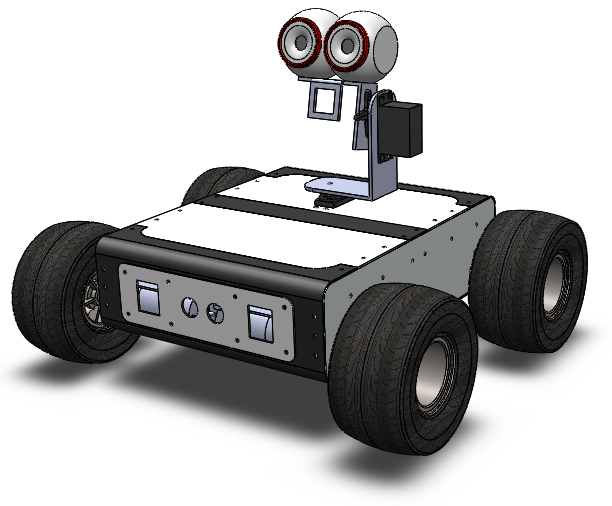
\includegraphics[width =.4\textwidth]{Fig/Introduction.png}
\caption{ A 3-D model for robot frame}
\end{figure}

%\clearpage

\subsection{History of Mobile Robots} 
Mobile robots have the capability to move around in their environment and are not fixed to one physical location. Mobile robots can be "autonomous" (AMR - autonomous mobile robot) which means they are capable of navigating an uncontrolled environment without the need for physical or electro-mechanical guidance devices. Alternatively, mobile robots can rely on guidance devices that allow them to travel a pre-defined navigation route in relatively controlled space (AGV - autonomous guided vehicle). By contrast, industrial robots are usually more-or-less stationary, consisting of a jointed arm (multi-linked manipulator) and gripper assembly (or end effector), attached to a fixed surface.\\
Mobile robots have become more commonplace in commercial and industrial settings. Hospitals have been using autonomous mobile robots to move materials for many years. Warehouses have installed mobile robotic systems to efficiently move materials from stocking shelves to order fulfillment zones. Mobile robots are also a major focus of current research and almost every major university has one or more labs that focus on mobile robot research. Mobile robots are also found in industrial, military and security settings. Domestic robots are consumer products, including entertainment robots and those that perform certain household tasks such as vacuuming or gardening. \cite{202}


\begin{figure}[H]
 \centering
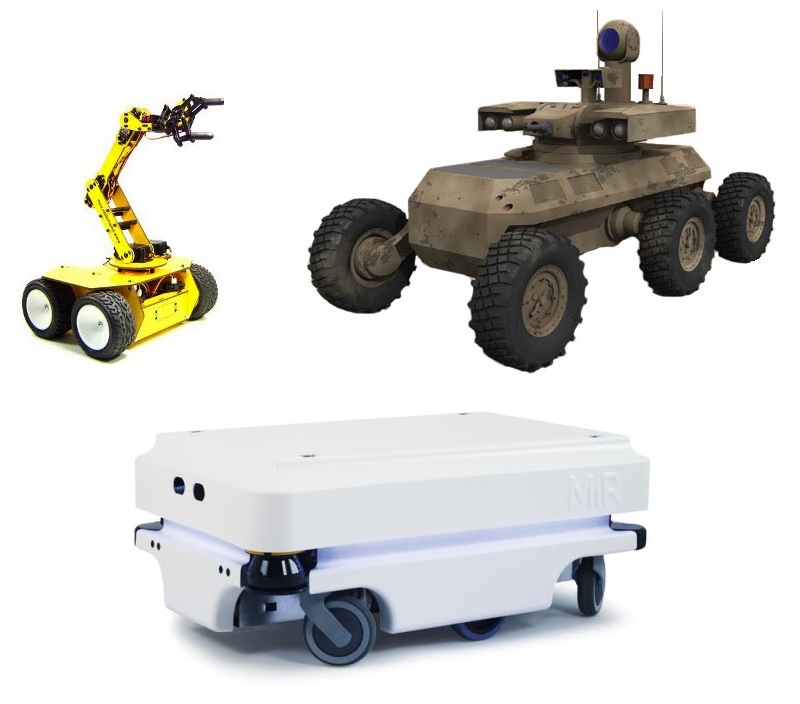
\includegraphics[width =0.6\textwidth]{Fig/mobile_robots_apps.jpg}
\caption{Different applications for mobile robots; industrial, military and transport}

\end{figure}

\subsection{Project Objectives}
The main objective of this project is to demonstrate a robust mobile robot in a small scale to perform an autonomous navigation from point to another. Also it is required for the robot to localize itself when asked to do. Both navigation and localization depends on the ability of robot to detect and recognize texts on landmarks that uniquely identifies specific nodes in the map.
For new environments whose map is not known, the robot can be guided remotely over the network to explore that location and a camera is provided for both steaming live video for the site around robot and to perform the computer vision task.
In the hardware level a robust controller is required to perform motion instructions with acceptable precision.

\newpage

\subsection{Limitations}
During our work we faced a lot of problems associated mostly with sensors. As we the main part in any control system is the feedback. This is because if we got a wrong indication for current state of system, we will perform a wrong reaction and the error increases more and more. In our project we need sensors to get information about the robot like position, velocity and orientation. Any missing part of them leads to both wrong estimation of state and wrong controller action.
In next sections we will talk about our trials, results and algorithms implemented to get the advantage of each sensor and avoid its misleading data.
\noindent But lets start from a high-level point of view and gradually take important topics with some details.

\subsection{Overview on the project parts}
The main system structure of our project as shown in figure \ref{fig:system-structure} consists of a GUI and controller box at user side and the master unit (RPi) at robot side. The operation starts from GUI to select the function needed and then a flow of communication commands are passed to master unit over the network to perform the required task. Controller box is used in manned mode of operation to guide robot motion and camera orientation. In next chapter we talk about the GUI; how you can use, how it is implemented and a quick over view on ROS (Robots Operating System).
\begin{figure}[H]
	\centering
	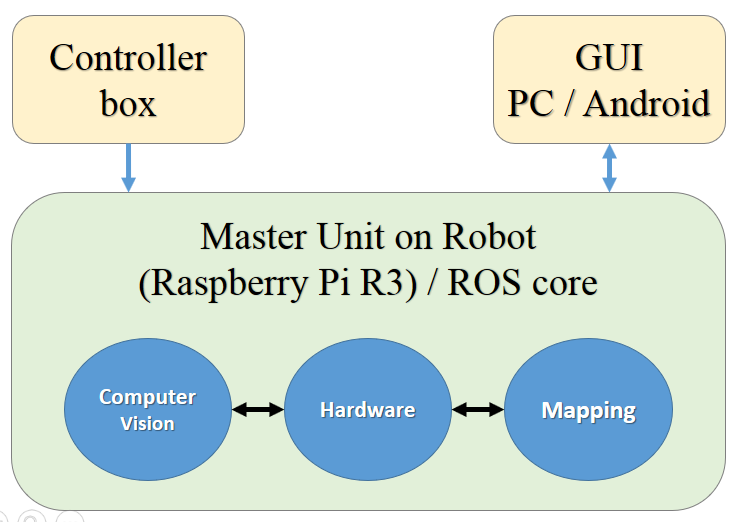
\includegraphics[width =0.6\textwidth]{Fig/overview.png}
	\caption{Clustered view of main system structure}
	\label{fig:system-structure}
\end{figure}
\newpage

\section{User Manual and GUI}
talk about how to use the GUI to run the project on different modes.

\newpage

\section{System Structure and Proposed Algorithm}
In the design stage of project, three main parts arises to be implemented; mapping, computer vision and hardware. Each part represents an executable program that can interact with other parts in a manner to fulfill the required task. So, lets first talk briefly about ROS and how it provided a great help in connecting project parts and how communication between processes becomes easy.



\subsection{Robots Operating System (ROS)}
The Robot Operating System (ROS) is a flexible framework for writing robot software. It is a collection of tools, libraries, and conventions that aim to simplify the task of creating complex and robust robot behavior across a wide variety of robotic platforms. \cite{201} \\
In ROS, Node is a common word that represents the executable file. So, in our project we have three main nodes; mapping, computer vision and hardware nodes. communication between nodes in ROS can be performed in many ways. The method we worked with is the message communication. Message represents the ROS data type. We developed a special type that can handle all communication needs between nodes. It is called Instruction and consists of a string variable that holds the command name and two float arguments. \\
Nodes can deal with messages in two manners; as a publisher, subscriber or both. Another word commonly used in ROS is the topic. It is considered as an intermediate program that holds any published message and forward it to all nodes that subscribed for it. This feature is very useful as a node can perform just one publishing command and any number of nodes can receive it. 
Now we know a bit about how ROS works and for more details and tutorials you can visit ROS tutorials site: http://wiki.ros.org/ROS/Tutorials. \\ \\
In next section we are to talk about our project nodes and how communication performed among them.
\begin{figure}[H]
	\centering
	
\includegraphics[width = 0.3\textwidth]{Fig/rosLogo.png}
	\caption{ROS logo.}
\end{figure}

\newpage

\subsection{Project Nodes and Communication Process}
As mentioned before, we have three main nodes; mapping, computer vision and hardware. the communication between them were created as shown in figure \ref{fig:nodes}. 
\begin{figure}[H]
	\centering
	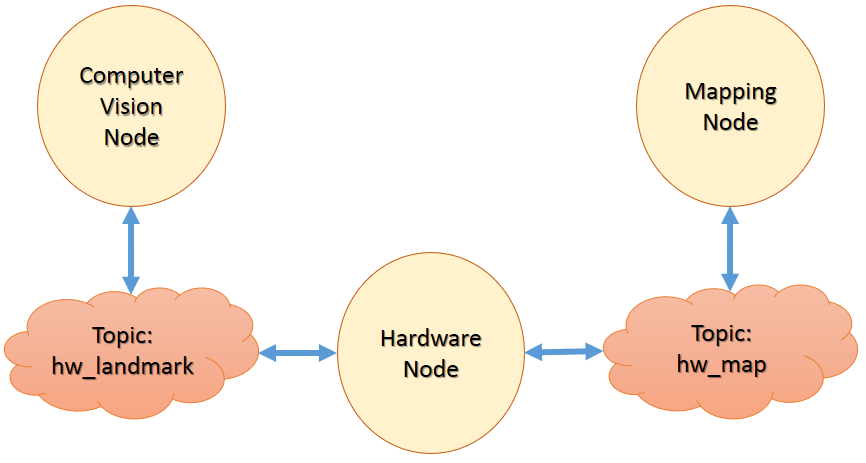
\includegraphics[width =0.6\textwidth]{Fig/Project-Nodes.png}
	\caption{The implemented nodes and advertised topics between them.}
	\label{fig:nodes}
\end{figure}
\noindent There are two advertised topics; hw\_landmark that connects hardware with computer vision and hw\_map that connects hardware to mapping node. Over the hw\_map topic the mapping node publishes the instructions that guide the robot from a landmark to another. When the robot reaches a new landmark, a tuning loop starts between hardware and computer vision node to put the robot exactly in front of the landmark. In this way, errors caused by inaccuracy of sensors or hardware motion performance are eliminated periodically resulting in a good autonomous navigation of the robot.\\
In next section we are to talk about the navigation algorithm and the sequence of instructions with some details.  




\subsection{Proposed Algorithm for Autonomous Navigation}
In the autonomous navigation mission, each of the three nodes has its own task to do. We can categorize these tasks in two phases. First phase is executed between Mapping and hardware node. Its goal is to guide the robot from one landmark to the next one on path to destination. Once the robot reaches that landmark or someplace near it, the second phase starts between computer vision node and hardware telling the robot how to move to stand exactly in front of the landmark. Figure \ref{fig:algorithm-phases} visualize these phases with brief description.

\begin{figure}
	\centering
	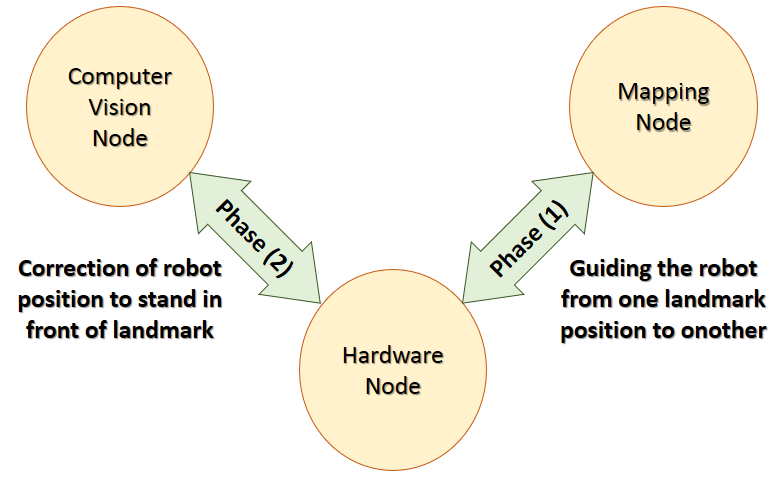
\includegraphics[width=0.7\textwidth]{Fig/Algorithm-phases.png}
	\caption{Proposed algorithm's phases}
	\label{fig:algorithm-phases}
\end{figure}

\noindent In the first phase, a sequence on instructions are passed from mapping to hardware node. These instructions can be 'move', 'rotate', 'rotate-camera' or a query for information of sensors. After each instruction the hardware responds by 'next\_step' command as an acknowledgment to mapping node that the last instruction is done. When the mapping node receives acknowledgment of last instruction, it sends a 'tune' command telling the robot to start the second phase. 

\noindent Second phase is a tuning process to eliminate any accumulated errors caused by hardware while performing mapping instructions. The computer vision node tries to guide the hardware to move in a way such that the land mark is detected at the center of picture frame. In this case, by knowing the distance between robot and wall we fully identify the robot position. Figure \ref{fig:localization} shows how localization is done by computer vision and range finder sensor.
\begin{figure}[H]
	\centering
	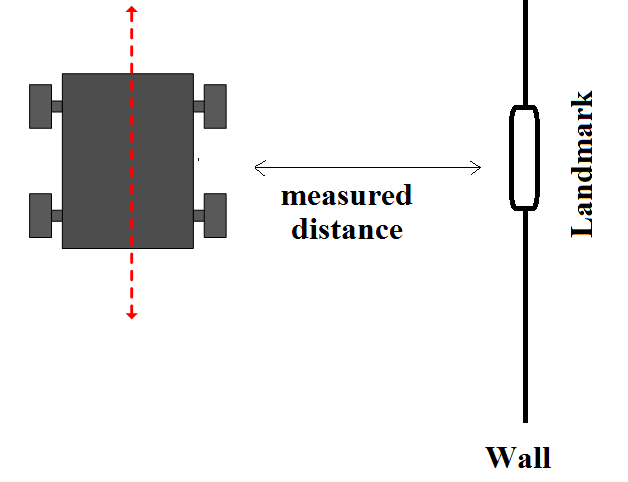
\includegraphics[width =0.4\textwidth]{Fig/localization.png}
	\caption{Localization using computer vision}
	\label{fig:localization}
\end{figure}

\noindent The flowchart of autonomous navigation process is provided ni figure \ref{fig:full-algorithm} showing the whole communication steps and conditions involved in such process. You can identify in this flowchart the role of each node and how it deals with others.

\newpage

\begin{figure}
	\centering
	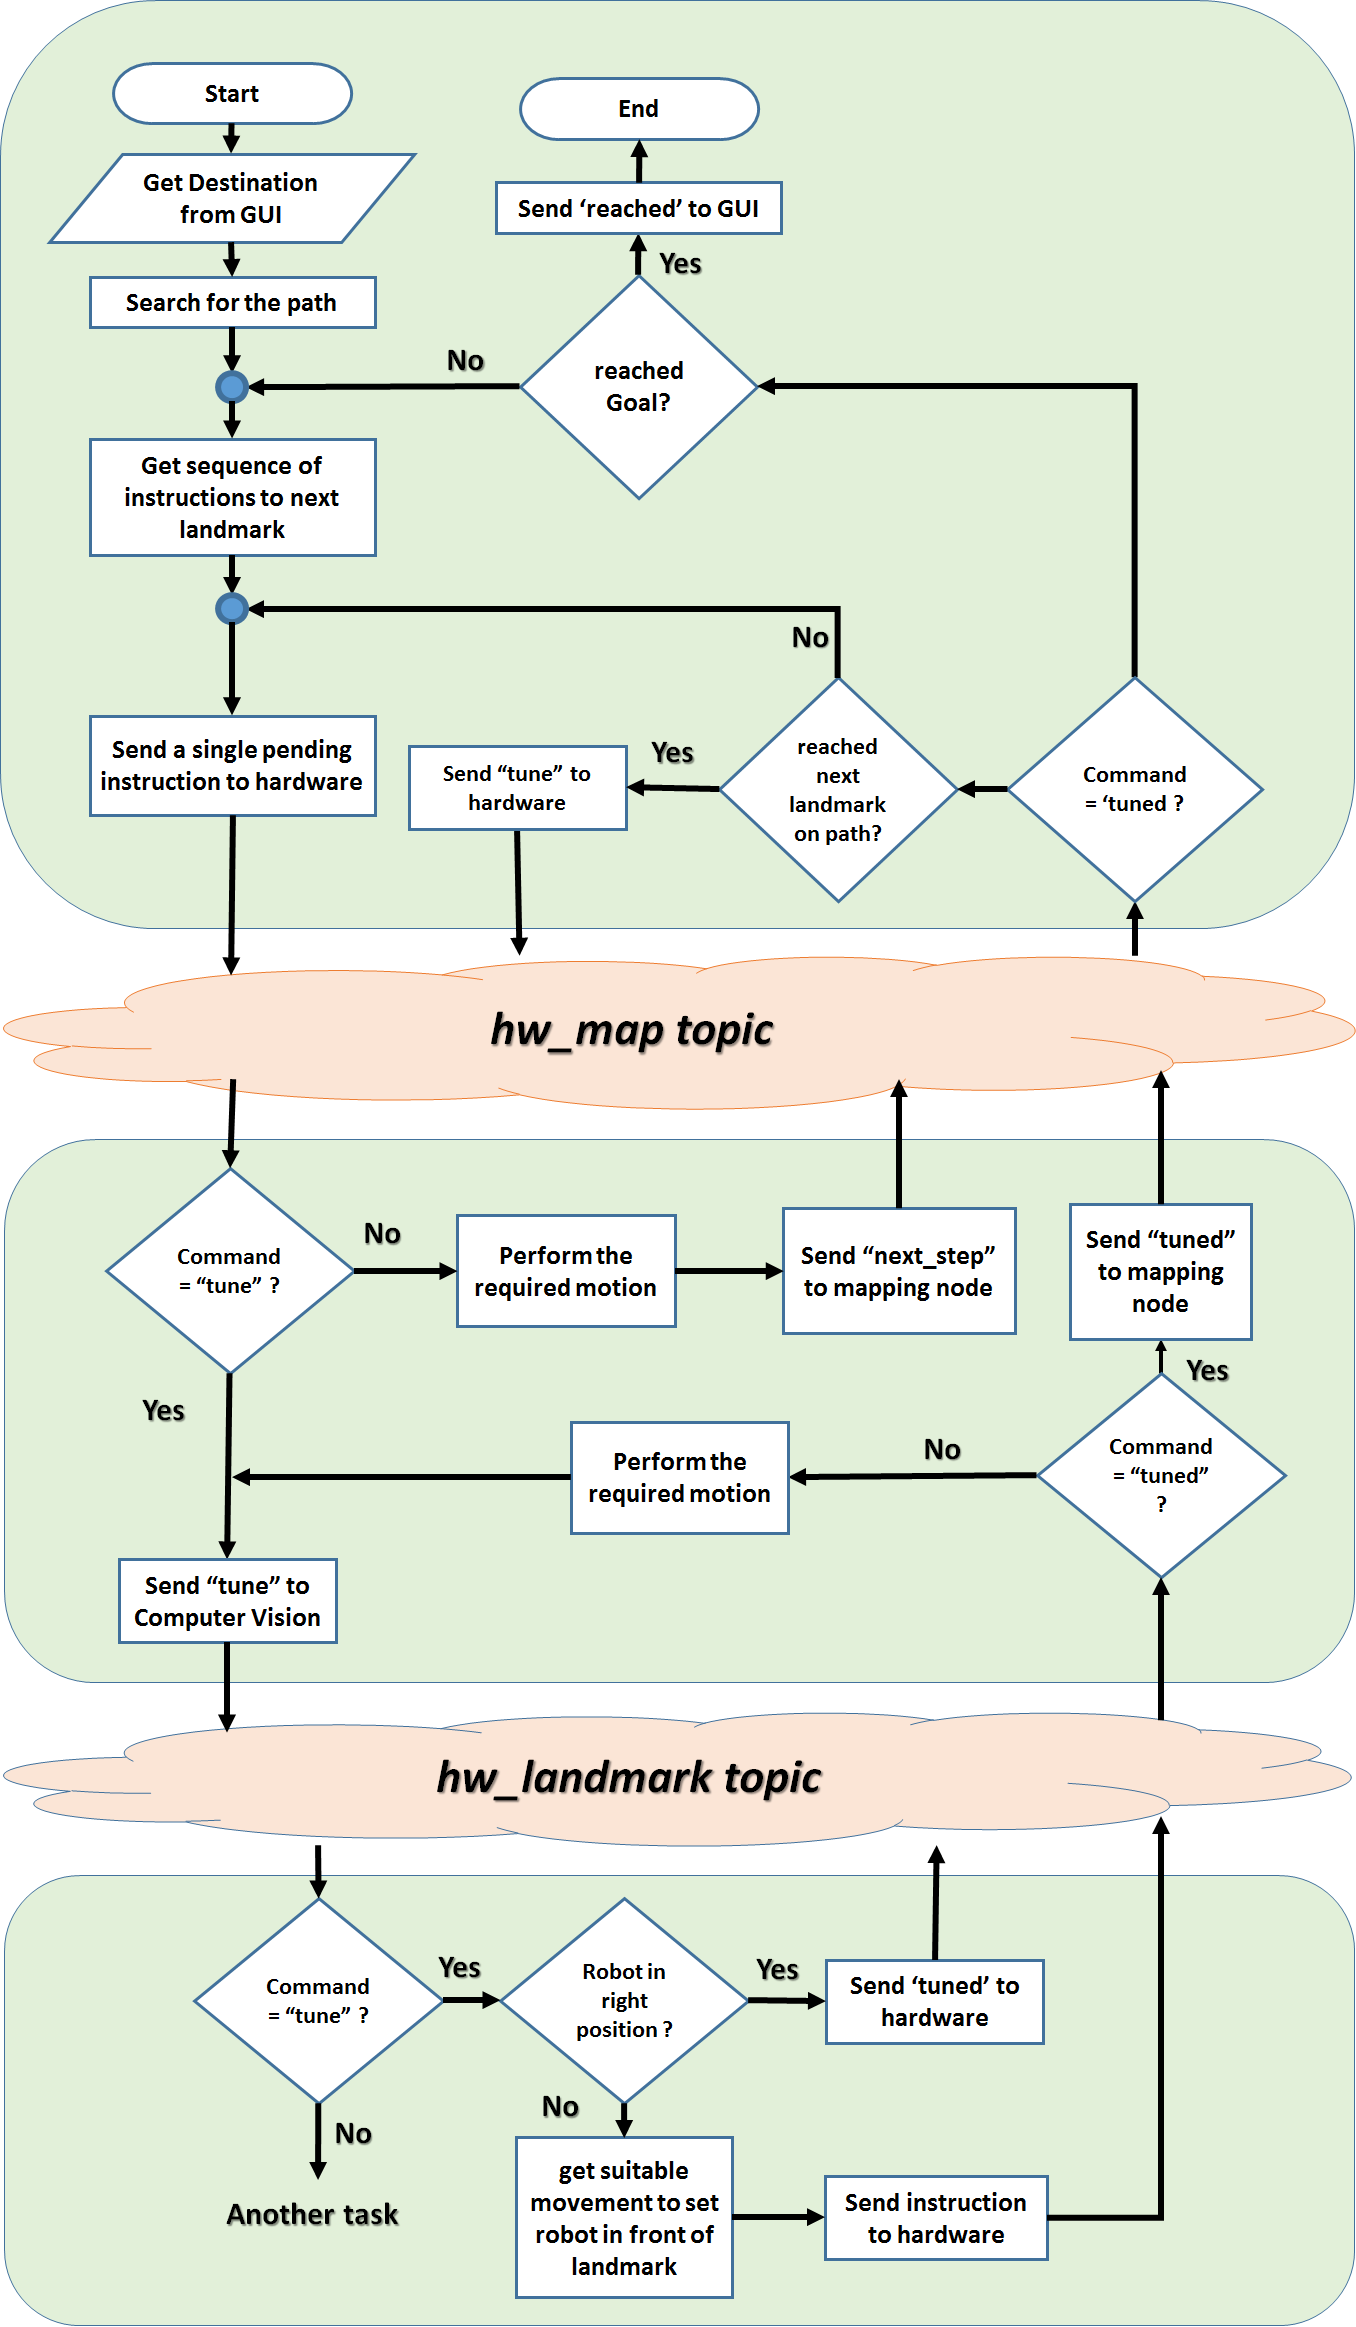
\includegraphics[width =0.75\textwidth]{Fig/full-algorithm.png}
	\caption{Flowchart for whole algorithm applied for autonomous navigation.}
	\label{fig:full-algorithm}
\end{figure}

\newpage
\clearpage
\newpage

\section{GUI Implementation}
talk about the Java application and how it is implemented, how it communicates with master unit to send navigation instruction. also how video stream is received

\newpage

\section{Mapping of Environment}
talk about graph theory and how map is represented. 
how landmarks are included in the map. 
Search algorithms.
instructions created to be sent to hardware.

\newpage

\section{Computer Vision}
talk about how detection, recognition and tuning are processed.

\newpage

\section{Hardware Node and Modules Structure Tree}
In prior sections we always look at hardware as a black box. This view is sufficient when we want to describe the overall operation of the robot. But lets now take this part in some details to know how instructions are processed after being received from either mapping or computer vision node. \\
In the design stage of hard ware, One of the most important aspects taken into consideration is modularity of design. Each Part in the hardware structure has a unique role and a method by which this role can be triggered for execution. Another important style of design followed is assigning low level tasks to multiple separate modules rather than having a central unit responsible for the whole operation. This method of design saves a lot of resources in the master unit opening the way for other complicated operations to be performed faster. In the following sections we will talk first about the role of hardware ROS node and then go down at low level.

\subsection{Hardware ROS node}
As mentioned in figure \ref{fig:full-algorithm} the hardware node stands midway between both mapping and computer vision nodes. its main role is receiving instructions from other nodes, refining them and forwarding them to low-level modules to be performed by robot. This leads to two important results. First, the hardware ROS node is free of low-level operations which keeps its main role of regarding and communicating with other nodes. Second, low level modules save their processing capability for optimized motion and performance rather than being concerned with communication of multiple parts. 
\begin{figure}[H]
	\centering
	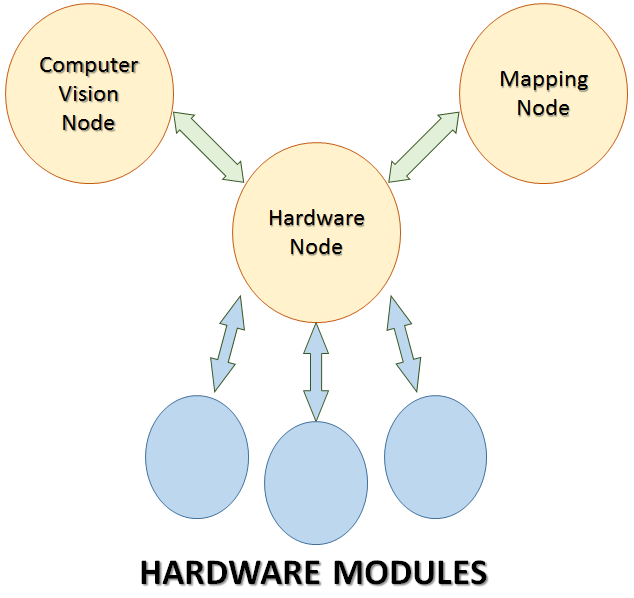
\includegraphics[width =0.45\textwidth]{Fig/hw-node.png}
	\caption{Hardware node standing midway between ROS nodes and hardware modules.}
	\label{fig:hw-node}
\end{figure}

\newpage

\subsection{Low-level Hardware Kits and Modules}
Here we reached to the stage of choosing the suitable kits and modules that can meet the needs of other nodes. In this case We must first encounter the whole instructions hardware may receive. These commands are as follow:
\begin{itemize}
	\item move straight some distance
	\item rotate robot some degrees
	\item set camera orientation
	\item measure distance between robot and any object around
	\item switch on flash light
	\item set motors speed
\end{itemize}
Each of these instructions has some requirements to be done. The modules we brought to fulfill these requirements can be encountered as follow:
\begin{center}
	\begin{tabular}{| c | c | c|}
		\hline
		Component & Function & Number of units \\
		\hline
		\hline
		Raspberry Pi R3 & Master Unit & 1\\
		\hline
		Arduino Nano Kits & processing units & 3\\
		\hline
		NodeMCU & micro controller with embedded WiFi module & 1\\
		\hline
		Motor driver & controlling motor speed and direction & 1\\
		\hline
		DC Motors & manipulators for robot motion & 4\\
		\hline
		Wheels & attached to motors & 4\\
		\hline
		Motor shaft encoder & counting revolutions of motor & 2\\
		\hline
		Compass Module & measuring heading angle & 1\\
		\hline
		Ultrasonic module & range finder & 4\\
		\hline
		Sharp IR sensor & range finder with longer distance span & 1\\
		\hline
		Camera & capturing the environment around & 2\\
		\hline
		Servo Motors & controlling camera orientation & 2\\
		\hline
		Lithium Battery & Power source for motors and Light & 1\\
		\hline
		Power bank 5V & Power source for Raspberry PI & 1\\
		\hline
		NiMH Battery 5V & Power source for Servo motors & 1\\
		\hline
	\end{tabular}
\end{center}

\noindent Components figures and data sheets are both included in appendix.

\newpage

\subsection{Hardware Tree Structure}
In this section we get closer to know how exactly project parts are connected to communicate. Also we will define the exact role for each part. As shown in figure \ref{fig:harware-structure} there are three sub nodes underlying the hardware node. Each one has sub-modules to control or communicate with. All these nodes are implemented on Arduino kits and this is a magnificent advantage for ROS as it provides libraries that enables us to implement ROS nodes on such kits.\cite{205} So, for each node it can publish and subscribe for message from the main hardware node on Raspberry Pi master. This enables us to have a single type of communication valid to use in all parts. We can identify the role of each node as follow:
\begin{itemize}
	\item \textbf{Manipulator Node:}\\
	This node is responsible for executing motion commands. The controller is implemented in this node. As we can see in figure \ref{fig:harware-structure} there three underlying parts, the motor driver, flash light and ultrasonic. You may wonder why ultrasonic is here in the manipulator node. This simply because we needed to summarize all parts that participate in the motion control in a single node to minimize the flow of communication message as possible. The motor driver has two tasks; sending speed signals to motors and combine the encoder pulses to the Arduino. More details about each module will be figured out in next sections.
	
	\item \textbf{Sensors Node:}\\
	
	
	\item \textbf{Manual Controller Box:}\\
	
	\begin{figure}[H]
		\centering
		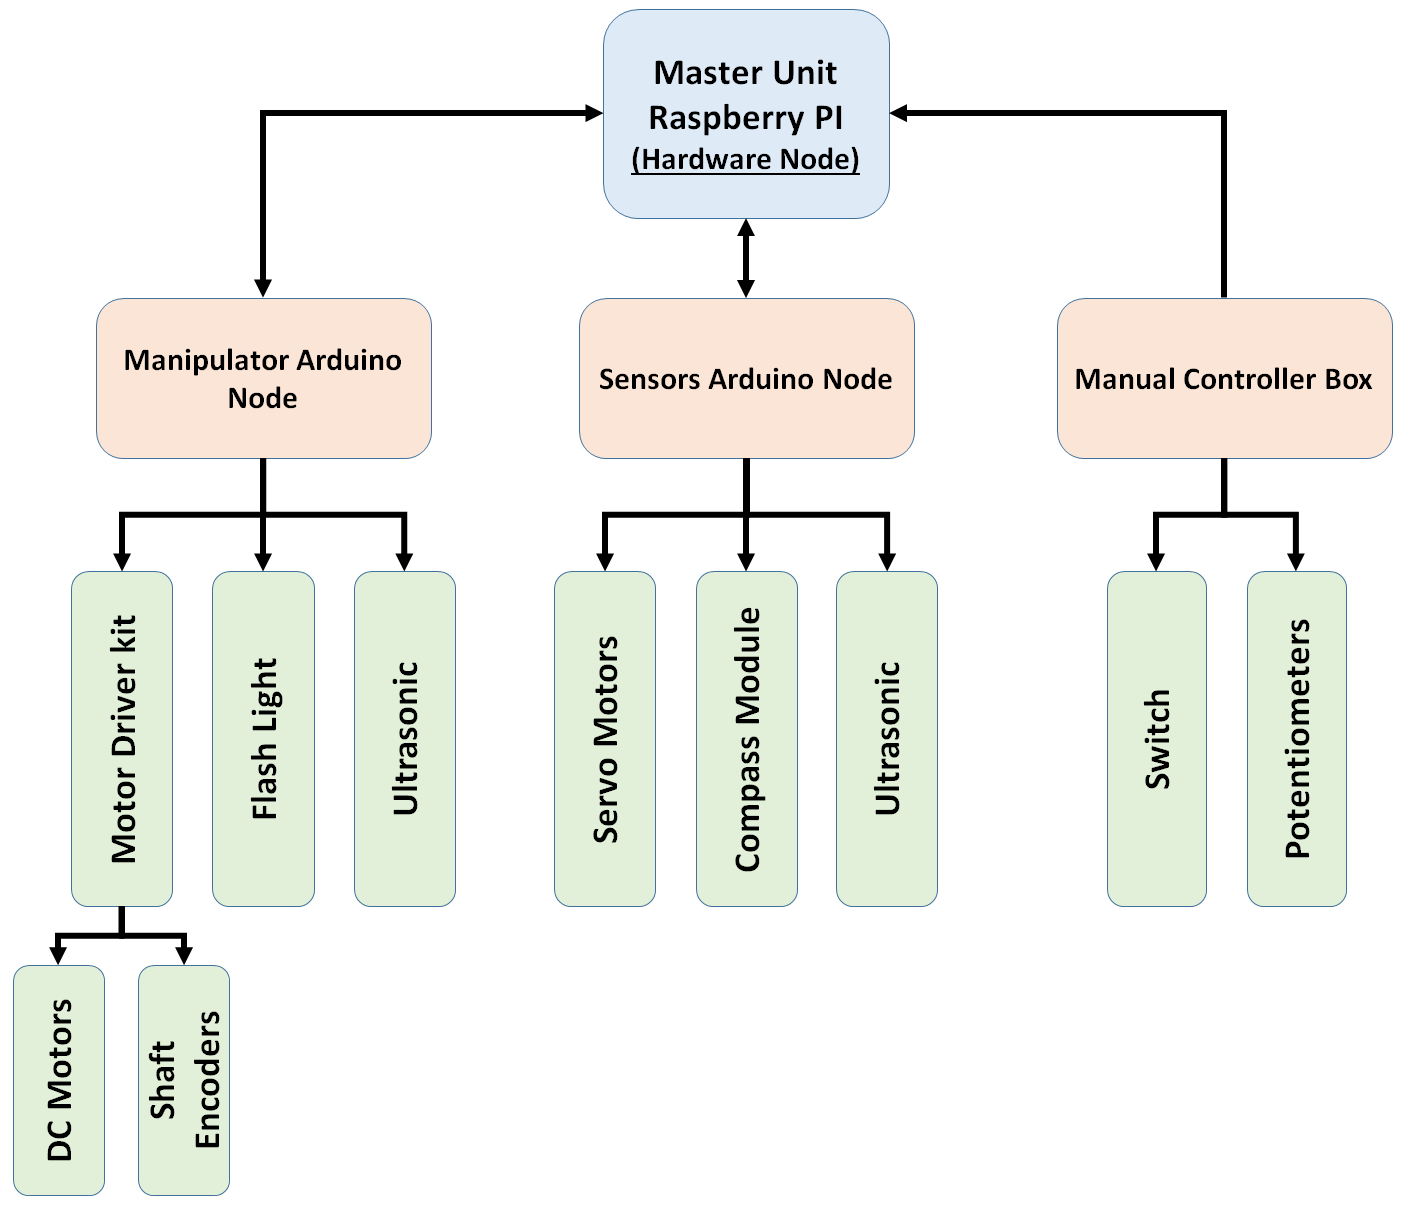
\includegraphics[width =0.9\textwidth]{Fig/hardware-structure.png}
		\caption{Hardware modules structure.}
		\label{fig:harware-structure}
	\end{figure}

	
\end{itemize}



\newpage

\section{Mechanical Design and Low-Level Control}
In this section we are about to take a close look on the design procedure of robot hardware both mechanical and electrical. The design stage of any application depends on the tasks and requirements it is supposed to fulfill. So, we will talk about functional requirements of project and how we select components to best suit them. Design engineers are usually constrained by one or more of these 5 concerns; time, money, knowledge, power and weight. So, there is no absolute good choice but we try to select the best one that meets the requirements and follow constraints. \cite{203} Then we will get a brief view on frame design, materials used and how manufacturing operation done. After that we will get closer to the low level control and talk about electronic modules and sensors used, function, advantages and disadvantages of each. Finally we reach the controller design; how it was implemented, tuned and tested.  

\subsection{Choosing Suitable DC Motor  \cite{203}}
In this project we introduce a robot for indoor navigation. So, in this case low speed is acceptable but at the same time it must be powerful enough for carrying and transporting most of parts we deal with at home or office. The requirements of robot were selected to be as follow:

\begin{itemize}
	\item \textbf{Functional Requirements:}
	\\ DC Gear head motor capable of accelerating a 20 Kg, four-wheel drive robot with wheel diameter of 6.5 cm at a rate of 1 ${m/s^2}$. Top speed required will be around 0.75 m/s. This speed is suitable as it reasonably approachs human walking speed.
	\item \textbf{Design Parameters:}
	\\Supplied Voltage = 12 V, Motor size limited to an overall diameter of approximately 4 cm and an overall length of not more than 10 cm (Less than robot frame width).
\end{itemize}
Here is the calculation steps based on the lecture notes referenced in section title:
\begin{itemize}
	\item \textbf{Step One: Calculating Required Torque and rpm:}
	\begin{itemize}
		\item \textbf{Required Torque:} \\
		${Force = Mass \times Acceleration}$\\
		${F_{total} = ma = 20 kg \times 1 m/s^2 = 20 N}$\\
		${F_w = F_{total} \div NumberOfWheels = 20 \div 4 = 5N }$\\
		${\tau = F d = F_w \times WheelRadius = 5 N \times 0.065 m = 0.325 Nm}$\\
		
		\newpage
		
		\item \textbf{Required rpm:}\\
		${Wheel Circumference = C_w = \pi D = 3.142 \times 0.13 m = 0.408m}$\\
		${Speed = RPS \times C_w}$\\
		${RPS = Speed \div C_w = 0.75 \div 0.408m = 1.838 rps = 110.294 rpm}$\\
		
	\end{itemize}
	
	\item \textbf{Step Two: Motor Selection to Meet the Requirements}\\
	After searching available electronics stores we got the most suitable motor for our project. Its model name is SG-555123000-30K shown in figure . From the data sheet provided for it find the following specs:\cite{204}
	\begin{itemize}
		\item Rated Voltage : 12 V
		\item No load Speed : 100 rpm
		\item Load torque speed : 73 rpm
		\item Torque : 0.34 Nm
	\end{itemize}
	By these specs we can conclude that robot features became as follow:
	\begin{itemize}
		\item ${Full  load  speed = rpm \times C_w \div 60 = 73 \times 0.408 \div 60 = 0.4964 m/s}$
		\item ${Pay load = \frac{ \tau_w \times 4}{ R_w \times a} = \frac{0.34 \times 4}{0.065 * 1} = 20.923 kg}$
		
	\end{itemize}
\end{itemize}

This is still acceptable speed because the robot is not supposed to work in full load all time. Moreover the speed of about 0.5 m/s is suitable also for indoor navigation purposes.

\begin{figure}[H]
	\centering
	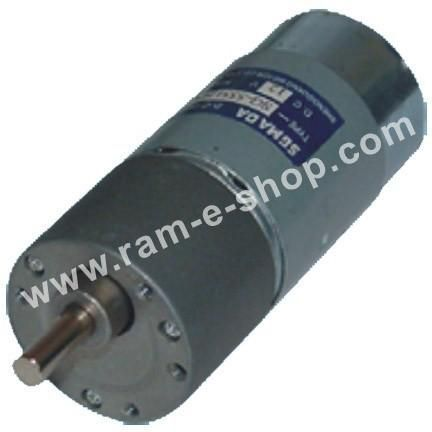
\includegraphics[width =0.35\textwidth]{Fig/dc-motor.jpg}
	\caption{DC motor SG-555123000-30K selected for driving the robot.}
	\label{fig:dc-motor}
\end{figure}



\newpage

\subsection{Robot Dimension and Solid Design}



mechanical analysis, solid design, final assembly, Motors choice.
Electric components, circuits, structure.
Sensors
Control system for straight line and rotation motion.

\newpage
\appendix

\section{Hardware modules and sensors}

\section{Solid Design Parts}

\newpage
 
\bibliographystyle{abbrv}
\bibliography{final}

\end{document}

